\chapter{\IfLanguageName{dutch}{Stand van zaken}{State of the art}}%
\label{ch:stand-van-zaken}

% Tip: Begin elk hoofdstuk met een paragraaf inleiding die beschrijft hoe
% dit hoofdstuk past binnen het geheel van de bachelorproef. Geef in het
% bijzonder aan wat de link is met het vorige en volgende hoofdstuk.

% Pas na deze inleidende paragraaf komt de eerste sectiehoofding.

% Dit hoofdstuk bevat je literatuurstudie. De inhoud gaat verder op de inleiding, maar zal het onderwerp van de bachelorproef *diepgaand* uitspitten. 
% De bedoeling is dat de lezer na lezing van dit hoofdstuk helemaal op de hoogte is van de huidige stand van zaken (state-of-the-art) in het onderzoeksdomein.
% Iemand die niet vertrouwd is met het onderwerp, weet nu voldoende om de rest van het verhaal te kunnen volgen, 
% zonder dat die er nog andere informatie moet over opzoeken \autocite{Pollefliet2011}.

% Je verwijst bij elke bewering die je doet, vakterm die je introduceert, enz.\ naar je bronnen. In \LaTeX{} kan dat met het commando \texttt{$\backslash${textcite\{\}}} of \texttt{$\backslash${autocite\{\}}}. Als argument van het commando geef je de ``sleutel'' van een ``record'' in een bibliografische databank in het Bib\LaTeX{}-formaat (een tekstbestand). Als je expliciet naar de auteur verwijst in de zin (narratieve referentie), gebruik je \texttt{$\backslash${}textcite\{\}}. Soms is de auteursnaam niet expliciet een onderdeel van de zin, dan gebruik je \texttt{$\backslash${}autocite\{\}} (referentie tussen haakjes). Dit gebruik je bv.~bij een citaat, of om in het bijschrift van een overgenomen afbeelding, broncode, tabel, enz. te verwijzen naar de bron. In de volgende paragraaf een voorbeeld van elk.

% \textcite{Knuth1998} schreef een van de standaardwerken over sorteer- en zoekalgoritmen. Experten zijn het erover eens dat cloud computing een interessante opportuniteit vormen, zowel voor gebruikers als voor dienstverleners op vlak van informatietechnologie~\autocite{Creeger2009}.

% Let er ook op: het \texttt{cite}-commando voor de punt, dus binnen de zin. Je verwijst meteen naar een bron in de eerste zin die erop gebaseerd is, dus niet pas op het einde van een paragraaf.

% \begin{figure}
%   \centering
%   \includegraphics[width=0.8\textwidth]{grail.jpg}
%   \caption[Voorbeeld figuur.]{\label{fig:grail}Voorbeeld van invoegen van een figuur. Zorg altijd voor een uitgebreid bijschrift dat de figuur volledig beschrijft zonder in de tekst te moeten gaan zoeken. Vergeet ook je bronvermelding niet!}
% \end{figure}

% \begin{listing}
%   \begin{minted}{python}
%     import pandas as pd
%     import seaborn as sns

%     penguins = sns.load_dataset('penguins')
%     sns.relplot(data=penguins, x="flipper_length_mm", y="bill_length_mm", hue="species")
%   \end{minted}
%   \caption[Voorbeeld codefragment]{Voorbeeld van het invoegen van een codefragment.}
% \end{listing}

% \lipsum[7-20]

% \begin{table}
%   \centering
%   \begin{tabular}{lcr}
%     \toprule
%     \textbf{Kolom 1} & \textbf{Kolom 2} & \textbf{Kolom 3} \\
%     $\alpha$         & $\beta$          & $\gamma$         \\
%     \midrule
%     A                & 10.230           & a                \\
%     B                & 45.678           & b                \\
%     C                & 99.987           & c                \\
%     \bottomrule
%   \end{tabular}
%   \caption[Voorbeeld tabel]{\label{tab:example}Voorbeeld van een tabel.}
% \end{table}

De volgende hoofdstukken geven een dieper inzicht in de volgende onderwerpen:
\begin{enumerate}
  \item Wat is warehousing, wat houdt automatisch warehousing in, en wat is de relatie met WCS en PLC?
  \item Overzicht van relevante communicatiemethoden die worden gebruikt door de PLC en het WCS.
  \item Uitleg van het verschil tussen asynchrone en synchrone communicatie, met een analyse van de voor- en nadelen.
  \item Vergelijking van de voor- en nadelen van cloud- en on-premise-oplossingen.
  \item Toelichting op verschillende communicatieprotocollen en messagingtechnologieën.
\end{enumerate}

\section{Inleiding tot Warehousing}
Omdat het onderzoek zich afspeelt in het domein van warehousing, wordt in dit hoofdstuk een algemeen overzicht besproken.
Warehousing of magazijnbeheer is het proces van het ontvangen, opslaan, beheren en verzenden van goederen in een specifieke omgeving. 
Magazijnen worden gebruikt voor een efficiënte doorstroom van materialen, waaronder grondstoffen, halffabricaten en eindproducten.
Material handling is een belangrijk onderdeel van warehousing, waarbij gebruik wordt gemaakt van apparatuur zoals 
transportbanden, heftrucks en automatische geleide voertuigen (AGV’s) om materialen door het magazijn te verplaatsen en te beheren.
\\
Binnen het magazijn vindt er een verscheidenheid aan activiteiten plaats, waaronder de ontvangst van goederen, 
het labelen en opslaan ervan, orderpicking en de uiteindelijke verzending naar klanten of productieafdelingen. 
Elk van deze stappen draagt bij aan een efficiënte bedrijfsvoering en zorgt ervoor dat producten veilig en op tijd beschikbaar 
zijn voor verdere verwerking of levering~\autocite{Berg1999}.
\\
TVH heeft het type distributie magazijn, waarbij verschillende producten van verschillende leveranciers verzameld  
en gebundeld worden zodat die efficiënt naar klanten kan gedistribueerd worden. 
Dit is een type dat vaak bij retailbedrijven en logistieke dienstverleners gebruikt wordt.
Verder kan je een distributie magazijn verdelen in twee soorten.

\begin{figure}
  \centering
  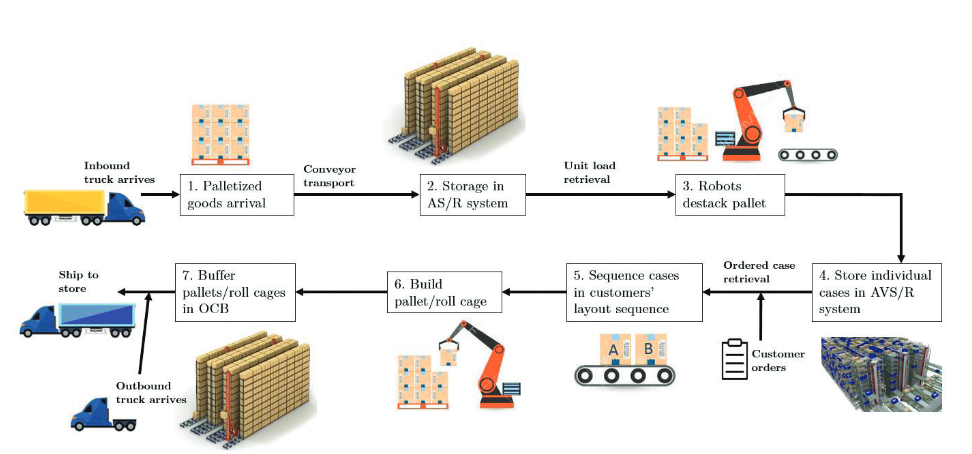
\includegraphics[width=0.8\textwidth]{../bachproef/img/warehousing_flow.png}
  \caption[Flow in a typical fully automated warehouse]{\label{fig:warehousing-flow}Standaard flow in een automatisch magazijn~\autocite{Koster2018}}
\end{figure}

\subsection{Handmatige systemen}
In deze soort beweegt de orderpicker zich naar de goederenlocaties, vaak met behulp van voertuigen zoals pickkarren of heftrucks. 
Deze systemen worden ook wel picker-to-product systemen genoemd, waarbij de medewerker fysiek de benodigde items verzamelt. 
Handmatige systemen zijn eenvoudig maar tijdrovend en vereisen veel arbeidskracht~\autocite{Berg1999}.

\subsection{Automatische systemen}
In deze systemen worden producten naar de orderpicker gebracht, vaak via ASRS-systemen (Automated Storage and Retrieval Systems). 
Dit zijn product-to-picker systemen waarbij de items automatisch worden verplaatst naar een vast pickpunt. 
Geautomatiseerde systemen kunnen de efficiëntie aanzienlijk verhogen door de reistijd van de orderpickers te verminderen 
en het picken te versnellen~\autocite{Berg1999}.
Het domein van dit onderzoek richt zich op het geautomatiseerde systeem. 

\section{Programmable Logic Controllers (PLC’s)}
Om een automatisch magazijn effectief aan te sturen, spelen Programmable Logic Controllers (PLC's) een cruciale rol.
PLC's zijn oorspronkelijk ontwikkeld om elektromechanische relais te digitaliseren in de industriële automatisering~\autocite{Bolton2015}. 
Door hun betrouwbaarheid, veelzijdigheid en robuustheid worden PLC’s breed toegepast in de industriële sector, waaronder in warehousing. 
In een magazijnomgeving monitoren en besturen PLC's tal van processen, zoals het transporteren van goederen, 
het positioneren van kranen en liften, en het uitvoeren van laad- en losactiviteiten.
Logistieke software wordt vaak gebruikt om bepaalde orders door te geven aan een PLC.

\subsection{Protocollen voor de communicatie van PLC's} 
De communicatie voor PLC’s kan worden gerealiseerd door middel van verschillende industriële protocollen, 
afhankelijk van de specificaties en vereisten van het magazijn en de gekozen hardware. 
Veelgebruikte protocollen zijn:

\subsubsection{Modbus}
Een relatief eenvoudig protocol dat oorspronkelijk ontwikkeld werd voor communicatie tussen PLC’s en sensoren of actuatoren. 
Het is een van de oudste protocollen en wordt nog steeds vaak gebruikt vanwege de eenvoud en lage kosten~\autocite{Joshi2024}. 

\subsubsection{Profinet}
Dit protocol biedt hoge snelheden en real-time communicatie 
en wordt vaak toegepast in grootschalige industriële automatiseringsprojecten, waaronder magazijnbeheer. 
Profinet is zeer geschikt voor situaties waarin hoge eisen worden gesteld aan nauwkeurigheid en stabiliteit.
Deze wordt gebruikt in het bedrijf om te communiceren tussen de PLC's.

\subsubsection{Ethernet/IP}
Dit protocol is gebaseerd op standaard TCP/IP en wordt veel gebruikt in de industrie vanwege de snelheid en flexibiliteit ~\autocite{Joshi2024}. 
Ethernet/IP ondersteunt real-time communicatie, wat essentieel is voor de snelle reactietijden die nodig zijn in een geautomatiseerd magazijn.
Dit protocol maakt gebruik van standaard Ethernet-hardware, zoals kabels, switches en routers. 
Dit vereenvoudigt de installatie en het onderhoud in industriële omgevingen en maakt het compatibel met bestaande IT-infrastructuur.
De PLC die deel uitmaakt van dit onderzoek, wisselt data uit van en naar het WCS via dit protocol.

\section{Warehouse Control System (WCS)} 
In het magazijn is de typische logistieke software het Warehouse Control System (WCS). 
Het WCS biedt een geïntegreerde interface voor een breed scala aan apparatuur waaronder de PLC's. 
Het systeem kan de apparatuur in het magazijn beheren en aansturen~\autocite{Son2015}. 
Binnen het bedrijf is het WCS een onderdeel van het monolithische ERP-pakket.

\section{Communicatie tussen WCS en PLC}
Een essentieel aspect van een geautomatiseerd magazijn is de soepele communicatie tussen de Programmable Logic Controllers (PLC’s) en 
het Warehouse Control System (WCS). 
Deze communicatie stelt het WCS in staat om gedetailleerde commando’s te sturen naar de PLC’s en om statusinformatie terug te ontvangen over de huidige staat van het magazijn en de apparatuur. 
Een stabiele en snelle datastroom tussen deze systemen is cruciaal voor een efficiënte werking en het minimaliseren van stilstand of fouten.
\\\\
Tijdens de samenwerking tussen PLC’s en het WCS worden er verschillende datastromen uitgewisseld via het Ethernet/IP netwerk.
Commando’s van WCS naar PLC: Het WCS stuurt instructies naar de PLC’s om specifieke handelingen uit te voeren, zoals het starten van een transportband of het positioneren van een kraan.
Statusupdates van PLC naar WCS: De PLC’s geven informatie terug aan het WCS over de huidige status van apparatuur. Bijvoorbeeld, of een transportband in werking is, 
de locatie van een item in het magazijn, en of er storingen of onderbrekingen zijn~\autocite{Laar2013}.
\\\\
Voor die communicatie wordt een middleware gebruikt van Progress OpenEdge, genaamd SonicMQ. 
Deze staat in als messaging broker, wordt niet meer actief ondersteund en wordt later besproken in de sectie message brokers.

\section{OpenEdge Progress 4GL} 
De software die gebruikt wordt voor de implementatie van het ERP-pakket en dus ook het WCS, is geschreven met OpenEdge Progress 4GL software.
Dit staat gekend onder OpenEdge ABL wat staat voor Advanced Business Language en is een high-level procedurele programmeer taal ontwikkeld door Progress Software Corporation.
Progress 4GL (Fourth-Generation Language) richt zich op bedrijfsapplicaties, vooral die met veel database-interacties~\autocite{OpenEdge2017}. 
Het biedt een vereenvoudigde syntaxis, waarmee ontwikkelaars snel toepassingen kunnen bouwen voor zakelijke omgevingen.
Dankzij de optimalisatie voor databasebewerkingen is het geschikt voor toepassingen in sectoren als financiën en logistiek, 
waar real-time datatoegang essentieel is.
 
\subsection{Progress OpenEdge JMS Adapter}
ABL applicaties zoals het WCS hebben een JMS (Java Messaging System) adapter nodig voor de communicatie met andere systemen, wat voorzien wordt door OpenEdge.
De adapter stelt OpenEdge-applicaties in staat om berichten te verzenden en te ontvangen van JMS message brokers zoals Apache ActiveMQ. 
Dit betekent dat OpenEdge-applicaties alleen kunnen integreren met messaging middleware die JMS ondersteunen. 
Een recente ontwikkeling (versie 12.8) maakt het mogelijk om Apache Kafka te integreren via een API die door OpenEdge wordt geleverd.
\\\\
De Progress OpenEdge JMS Adapter biedt twee methoden voor het verbinden met een message broker: Client Connect en Broker Connect.
\subsubsection{Broker Connect}
Is een methode waarbij de communicatie wordt gemaakt via een tussenlaag. Services verbinden via een specifieke poort op de communicatie server
dat de verbinding met de messaging broker beheerd. Dit is voordelig voor de veiligheid omdat de JMS broker niet rechtstreeks blootgesteld wordt.
De opzet van deze methode kan complexer zijn dan Client connect.

\subsubsection{Client Connect}
Deze methode verbind direct met de messaging broker waardoor integratie eenvoudiger is. 
Hierdoor is de message broker rechtstreeks blootgesteld op het netwerk.


\section{Communicatie methodes}
Dit hoofdstuk bevat informatie over de relevante communicatiemethoden en geeft inzicht in hun werking.
Deze methodes kunnen zowel on-premise als on-cloud gebruikt worden door het IT infrastructuur.
\\
\emph{Inter-Process Communication (IPC)} omvat alle vormen van communicatie tussen services, 
zowel binnen hetzelfde systeem als via een netwerk. 
Hieronder worden enkele methoden van \emph{Message Passing} toegelicht.

\subsection{Socket gebaseerd (TCP/UDP)}
Een socket-verbinding (TCP/IP) maakt gebruik van een endpoint gespecificeerd met een IP-adres en een poortnummer, 
waarmee twee autonome processen verbonden zijn, hetzij op dezelfde, hetzij op verschillende machines.
\\
\textbf{Streaming sockets} (op basis van TCP) zijn nuttig voor betrouwbare, sequentiële berichtoverdracht.
Deze methode wordt gebruikt voor de connectie tussen de PLC en het WCS.
\\ 
\textbf{Datagram sockets} (op basis van UDP) zijn geschikt zijn voor snelle, maar minder betrouwbare communicatie en wordt gebruikt voor bijvoorbeeld audio en video.
Beiden ondersteunen communicatie tussen verschillende netwerken en zijn veelgebruikt~\autocite{Dinari2020}.

\subsection{Message queue-gebaseerd}
Deze vorm van communicatie kent twee fundamentele modellen die de basis vormen voor de werking van een messaging-systeem. 
Afhankelijk van de gekozen message broker worden verschillende protocollen toegepast. 
Deze worden later besproken.

\subsubsection{Publish-subscribe-model}
Het publish-subscribe-model is gebaseerd op \textbf{topics} waarop berichten worden gepubliceerd door de \emph{producer} 
en waar meerdere \emph{subscribers} (abonnees) zich kunnen op inschrijven~\autocite{Dinari2020}. 
\\
In een op \emph{topic} gebaseerd systeem worden berichten geplaatst in \emph{topics} wat logische kanalen zijn.
\emph{Subscribers} ontvangen berichten van de \emph{topics} waarop ze zich hebben geabonneerd.
Alle \emph{subscribers} ontvangen dezelfde berichten uit dezelfde \emph{topics}. 
Deze methode zorgt voor een \textbf{one-to-many} vorm van communicatie~\autocite{Dinari2020}.
\\
Hierdoor ontvangen subscribers alleen de berichten uit de klassen die voor hen relevant zijn, zonder enige kennis van de publishers. 
Met het publish-subscribe-model specificeert de afzender nooit expliciet wie de ontvanger is en weet het zelfs niet of er al dan niet ontvangers zijn.

\begin{figure}[h!]
  \centering
  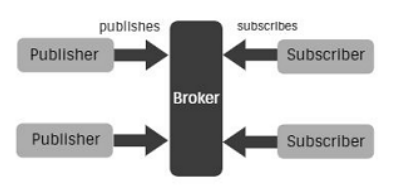
\includegraphics[width=.4\textwidth]{../voorstel/img/fig1-publish-subscribe.png}
  \caption{\label{fig:pub-sub}Publisher-Subscriber system~\autocite{Sharvari2019}}
\end{figure}

\subsubsection{Point-to-Point-model}
Hier worden berichten door \emph{publishers} in specifieke wachtrijen geplaatst, 
genaamd \textbf{queues} waarna andere nodes, genaamd \emph{consumers} ze eruit halen. 
\\
Messaging queues hebben een asynchrone werking, zijn \emph{socket-based} en maken gebruik van \emph{message queuing}, 
waarbij het de \textbf{point-to-point} methodiek gebruikt.
Hierbij plaatst de \emph{producer} berichten in een specifieke queue, waarna een \emph{consumer} de berichten uitleest in een sequentiële volgorde.
Met andere woorden, een bericht wordt slechts aan één \emph{consumer} bezorgt.
\\
Dit maakt het voor applicaties mogelijk om asynchroon te communiceren zonder te moeten wachten op een antwoord van de ontvanger.
Ze zijn geschikt voor gedistribueerde systemen waar processen onafhankelijk werken~\autocite{Dinari2020}.

\begin{figure}[h!]
  \centering
  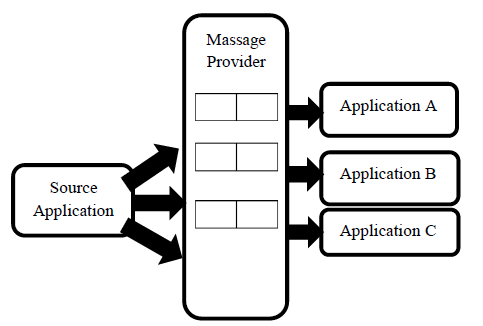
\includegraphics[width=.4\textwidth]{../bachproef/img/point-to-point-messaging.png}
  \caption{\label{fig:point-to-point}Point-to-point system~\autocite{Dinari2020}}
\end{figure}

% \subsection{Niet relevante methodes}

% \subsubsection{RPC-methoden voor messaging}
% In dit hoofdstuk worden de \emph{Remote Procedure Call} (RPC) methoden besproken. 
% Deze communicatiemethode is synchroon, wat betekent dat de verzendende partij moet wachten op een antwoord.
% Hierdoor is deze manier van communiceren niet optimaal voor het domein van dit onderzoek, 
% aangezien het niet de vereiste prestaties levert. 
% Desondanks worden deze methoden besproken om inzicht te geven in hoe ze werken en om aan te tonen waarom ze niet geschikt zijn.

% \subsubsection{XML en SOAP}
% Deze methoden zijn relevant voor communicatie omdat ze methoden en objecten via XML over HTTP kunnen aanroepen,
% wat communicatie mogelijk maakt tussen verschillende platformen en programmeertalen.
% Zoals eerder besproken zijn deze synchroon waardoor de snelheid nadelig beïnvloed wordt.

% \subsubsection{REST}
% RESTful webservices gebruiken HTTP-verzoeken (zoals GET, POST) voor eenvoudige en efficiënte berichtuitwisseling en is heeft ook een synchrone werking. 
% De berichten, meestal in JSON formaat, maakt dit geschikt voor communicatie tussen webapplicaties.

% \subsubsection{Pipes}
% \textbf{Named pipes} hebben een synchrone werking en voorzien een bidirectionele 
% communicatie tussen onafhankelijke processen.
% Deze maakt het mogelijk om te kunnen functioneren tussen processen op hetzelfde systeem.
% \\
% \textbf{Ordinary pipes} bieden beperkte eenzijdige communicatie en vereisen een parent-child relatie, 
% wat ze minder geschikt maakt voor communicatie tussen onafhankelijke processen~\autocite{Dinari2020}.

% \subsubsection{Shared memory}
% Deze methode is niet relevant voor dit onderzoek omdat het gericht is op het delen van geheugenruimte 
% tussen processen op hetzelfde systeem. 
% Ze zijn nuttig voor het efficiënt delen van grote hoeveelheden data binnen hetzelfde systeem~\autocite{Dinari2020}.

\subsection{Synchroon vs. asynchroon}
Services communiceren zowel \emph{synchroon} als \emph{asynchroon} en spelen deze benaderingen een cruciale rol, 
elk met hun eigen voor- en nadelen. \emph{Synchrone microservices} werken volgens een direct 
afhankelijkheidsmodel, omdat services met elkaar communiceren in een vraag-antwoordpatroon. 
\\\\

\textbf{Synchrone} communicatie kan leiden tot ingewikkelde onderlinge afhankelijkheden, vertragingen en complexiteiten bij het debuggen 
van de logica. Bovendien wordt het schalen van synchrone services uitdagend, 
aangezien de schaalbaarheid van één service sterk afhankelijk is van andere services die het gebruikt \autocite{Bellemare2020}.  
\\\\

\textbf{Asynchrone} communicatie heeft een reeks voordelen. Ze bieden grotere schaalbaarheid, technologische 
flexibiliteit en aanpassingsvermogen aan veranderende zakelijke vereisten. 
In plaats van de synchrone manier van communicatie is de \emph{asynchrone} gemakkelijker te herstructureren en te onderhouden. 
Ze vergemakkelijken \emph{continuous delivery} door hun onafhankelijkheid omdat de communicatie 
met een \emph{messaging systeem} opgevangen wordt. 
Hun verminderde afhankelijkheden en geïsoleerde karakter maken het testen relatief eenvoudiger en robuuster.
Het enige grote nadeel in asynchrone communicatie is \emph{error handling}, 
omdat dit niet opgevangen kan worden door de verzendende partij.
\newline

\begin{figure}[h!]
  \centering
  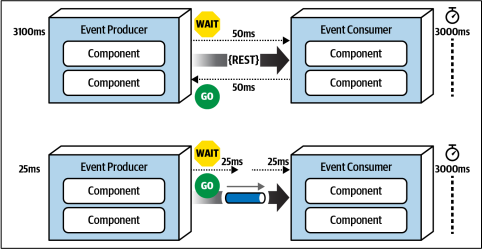
\includegraphics[width=.5\textwidth]{../voorstel/img/synchronous_vs_async_calls.png}
  \caption{\label{fig:sync-vs-async}Synchronous versus asynchronous communication \autocite[figure 14 -- 13]{MarkRichards2021}.}
\end{figure}

In praktische termen is het vinden van de juiste balans tussen \emph{synchrone} en \emph{asynchrone microservices} cruciaal, 
afhankelijk van de specifieke behoeften van een organisatie en de aard van haar bedrijfsprocessen. 
Een hybride aanpak waarin beide architecturen naast elkaar bestaan en elkaar aanvullen blijkt vaak de meest effectieve strategie te zijn. 
Deze aanpak stelt organisaties in staat om de sterke punten van zowel synchrone als asynchrone modellen te benutten, 
waardoor flexibiliteit, schaalbaarheid en onderhoudsgemak worden gegarandeerd in complexe \newline IT-landschappen.
In deze paper ligt de focus op \emph{asynchrone communicatie} voor het gebruik van \emph{messaging systemen}.
\newline

\subsection{Cloud vs. On-premise}
Dit hoofdstuk vergelijkt cloud- en on-premise-oplossingen, waarbij de verschillen, voordelen en uitdagingen van beide opties worden belicht. 
De huidige setup in het bedrijf voor de communicatie tussen PLC en WMS is on-premise opgesteld.
Cloud-oplossingen draaien op externe servers die via het internet toegankelijk zijn, 
terwijl on-premise-oplossingen lokaal binnen de eigen infrastructuur worden beheerd en onderhouden.
De snelheid over het netwerk kan onderzocht en getest worden voor beide toepassingen en is relevant voor het aanbevelingsrapport.
Volgend overzicht is een samenvatting uit een onderzoek van \cite{Golec2021} en van \cite{Fisher2018}:

\textbf{Cloud:}
\begin{itemize}
  \item Flexibiliteit: Hardware, software en applicaties extern beheerd door een serviceprovider.
  \item Kosten: organisaties betalen alleen voor de gebruikte resources. Dit kan hoger oplopen op langere termijn. 
  \item Beveiliging: Cloud biedt uitgebreide beveiligingsmaatregelen en beleidsregels, inclusief speciale cloud omgevingen voor gevoelige data.
  \item Onderhoud: wordt volledig door de cloud provider verzorgd, inclusief automatische updates en upgrades.
  \item Schaalbaarheid: infrastructuur kan snel worden aangepast aan veranderende behoeften, wat sneller en eenvoudiger is dan bij on-premises modellen.
\end{itemize}

\textbf{On-Premise:}
  \begin{itemize}
    \item Flexibiliteit: Hardware, software en applicaties op locatie in het eigen datacenter, wat meer controle en verantwoordelijkheid vereist.
    \item Kosten: brengen hogere initiële kosten met zich mee voor hardware en software maar is op langere termijn goedkoper.
    \item Beveiliging: is volledig in eigen handen, wat een voordeel kan zijn, maar ook extra zorg en middelen vereist.
    \item Onderhoud: organisaties zijn verantwoordelijk voor het onderhoud van servers, data-back-ups en disaster recovery
    \item Schaalbaarheid: is beperkter, het aanpassen van de infrastructuur of het uitbreiden van servers is een tijdrovend proces in vergelijking met de cloud
  \end{itemize}
   
\begin{table}[!h]
  \centering
  \begin{tabular}{lcc}
    \toprule Kenmerk & Cloud & On-Premise \\
    \midrule Kosten & Pay-per-use & Hoge initiële investering \\
    Beheer & Cloud provider & Eigen organisatie \\
    Schaalbaarheid & Gemakkelijk & Beperkt \\
    Beveiliging & Uitgebreide maatregelen & Eigen verantwoordelijkheid \\
    Toegankelijkheid & Van overal & Beperkt tot lokaal netwerk \\
    Onderhoud & Door cloud provider & Eigen verantwoordelijkheid \\
    Performance & Meestal hoog & Hoog \\
    Beschikbaarheid & Hoog & Eigen verantwoordelijkheid \\
    \bottomrule
  \end{tabular}
  \caption{\label{tab:cloud_vs_onpremise}Vergelijking tussen Cloud en On-Premise oplossingen\autocite{Golec2021}}
\end{table}

\section{Messaging protocollen}
In dit hoofdstuk worden de meest relevante messaging protocollen besproken die later in het vergelijkend onderzoek aan bod komen.

\subsection{AMQP (Advanced Message Queuing Protocol)} 
AMQP is een protocol gebaseerd op het publish-subscribe model, een veelgebruikt protocol in de huidige IT infrastructuur.
Het belangrijkste doel van AMQP is het bieden van betrouwbaarheid bij het verzenden van berichten \autocite{Adiono2020}.  

\subsubsection{Hoofdfuncties van AMQP}
AMQP wordt ook gebruikt als standaard voor messaging. 
Het AMQP-protocol wordt als meer compatibel beschouwd met onstabiele internetverbindingen omdat het een store-and-forward functie heeft. 
Deze functie kan gegevens tijdelijk opslaan als de verbinding onstabiel is of tijdelijk uitvalt. 
AMQP heeft ook een goede interoperabiliteit, omdat het multi-user, multi-infrastructuur, flexibele routing en beveiliging kan bieden.
 
\subsubsection{Toepassingen}
AMQP wordt gebruikt in uiteenlopende domeinen die belang hechten aan betrouwbaarheid, waaronder:
\\
\textbf{Autonome systemen:} Voor het coördineren van gedistribueerde processen. \\ 
\textbf{Cloud computing:} Voor veilige en gestructureerde gegevensoverdracht.  \\
\textbf{IoT-technologie:} Voor het waarborgen van betrouwbare communicatie en veiligheidsaspecten in IoT-apparaten.

\subsection{MQTT (Message Queue Telemetry Transport)}
MQTT is een publish/subscribe service protocol dat gebruikmaakt van een infrastructuur waarin clients verbinding maken met een centrale server, de zogenaamde broker. 
Het protocol kent drie essentiële componenten: de publisher, de subscriber, en de server (broker)~\autocite{Usmani2021}.

\subsubsection{Hoofdfuncties van MQTT}
De publisher creëert data en plaatst deze op een topic dat dan door de broker gedistribueerd wordt naar relevante ontvangers.
De subscribers zijn de eindgebruikers van de gegevens. Deze ontvangen de data via de broker om te verwerken.
De broker coördineert de gegevensuitwisseling tussen publishers en subscribers en fungeert als de centrale infrastructuur.

\subsubsection{Toepassingen}
Het protocol vereist weinig bandbreedte en energie, dankzij de kleine headergrootte. 
Dit maakt het zeer geschikt voor IoT-apparaten.

\textbf{Industriële Automatisering (IIoT):} Apparaten in fabrieken of pijpleidingen communiceren met centrale systemen voor real-time monitoring.
\textbf{Gezondheidszorg:} Monitoring op afstand van patiënten via draagbare apparaten zoals glucosemeters of hartslagmonitors.
\textbf{Transport en Logistiek:} Beheer van voertuiglocaties en conditie van vracht zoals temperatuur van gekoelde opslag.
 
\section{Message brokers}
Message brokers zijn middleware die instaan voor de communicatie via publish/subscribe-queues tussen verschillende services.
Producers sturen een bericht naar de broker door gebruik te maken van een bepaald protocol.
De functie van een message broker is het opslaan op een wachtrij (queue), routeren en versturen van een bericht.
Berichten worden opgepakt door de consumer dat zich ingeschreven heeft op berichten met een bepaald onderwerp.
Nadat een bericht is verwerkt door de consumer, wordt deze verwijderd.

\section{EoL Systemen}
Wat?\\
Waarom gevaarlijk?\\

 










